% !TeX root = ../tfg.tex
% !TeX encoding = utf8

\chapter{Extracción de datos radiómicos y machine learning clásico} \label{chap:aa-radiomica}

En este capítulo se describe el procedimiento realizado para el entrenamiento de modelos de aprendizaje automático a partir de características radiómicas como las definidas en la Sección \ref{sec:radiomica}.

El aprendizaje con características radiómicas es una estrategia que se utiliza comúnmente en problemas médicos \parencite{shur2021radiomics,mukherjee2022radiomics}. Esto se debe a muchos factores. Por un lado, las características que se extraen son explicativas y pueden ser interpretadas por los médicos. Por otra parte, estos atributos se pueden entrenar con modelos de aprendizaje clásico no paramétricos o con una cantidad de parámetros reducida, haciendo posible un aprendizaje efectivo con una cantidad de datos menor que la que requerirían otros modelos, como los de aprendizaje profundo. También, puesto que estas características se extraen como datos tabulares, la integración con otros tipos de datos, como los datos clínicos, se hace inmediata.

En las siguientes secciones se mostrará qué características se han extraído y qué preprocesamientos de imágenes se han elegido para extraer características. Se hará un breve análisis y preselección de estas y se analizarán distintos preprocesamientos, para finalmente poder entrenar varios modelos de aprendizaje diferentes. Se analizará tanto la consideración únicamente de características radiómicas, como la combinación de estas con los datos clínicos. Adicionalmente, se concluirá el capítulo describiendo una aproximación basada en aprendizaje de métricas de distancia dado el buen rendimiento inicial que mostró el clasificador $k$-NN en la primera aproximación que se realizó en esta experimentación.

\section{Extracción de características radiómicas}

Para la extracción de características radiómicas se ha utilizado la biblioteca de Python \texttt{pyRadiomics} \parencite{van2017computational}, una biblioteca de código abierto con una extensa funcionalidad para extraer características de todos los tipos y con amplias opciones de parametrización. 

El software requiere objetos de imagen para trabajar, no basta con cargar una matriz de vóxels, ya que los archivos DICOM o NIfTI almacenan metadatos adicionales de información espacial, que son importantes en el proceso de extracción. Para ello, se ha hecho uso también de la biblioteca \texttt{SimpleITK} \parencite{yaniv2018simpleitk}, especializada en la lectura y escritura de imágenes médicas multidimensionales en Python. Además de las imágenes, \texttt{pyRadiomics} admite especificar una región de interés específica dentro de la imagen que se utilice para la extracción de características, mediante una máscara binaria.

En nuestro problema particular, se ha aplicado el software sobre todos los volúmenes NIfTI usando como máscara la segmentación a nivel de pulmón proporcionada por \texttt{TotalSegmentator}, evitando así que el extractor de características se fije en detalles exteriores al pulmón. Una vez extraídas las características de los pacientes, se genera un archivo \texttt{CSV}, donde cada fila representa un paciente (en la primera columna se guarda el índice del paciente), y las columnas representan todas las características que proporciona el extractor para la imagen de TC de cada paciente.

El algoritmo de extracción se ha ejecutado con varios parámetros que se suelen usar habitualmente en este tipo de problemas:

\begin{itemize}
    \item \texttt{binWidth}: define la anchura de intervalo en los histogramas que se usan para las características de textura. Se ha usado un valor de 25.
    \item \texttt{resampledPixelSpacing}: indica cómo remuestrear la imagen, para uniformizar los volúmenes en los que las longitudes de los cortes, o equivalentemente, el tamaño de los vóxels, son diferentes. Se ha usado un remuestreo del tamaño de vóxel a $[1, 1, 1]$ mms.
    \item \texttt{interpolator}: indica qué interpolación usar en el remuestreo anterior. En este caso se hace mediante un B-Spline.
    \item \texttt{normalize}: indica si aplicar normalización estándar a las intensidades dentro de la región de interés. Puede ayudar a evitar errores de calibración de los escáneres. Se ha activado en esta experimentación.
    \item \texttt{removeOutliers}: establece un umbral para el cual no se consideran determinadas intensidades outliers en la normalización. Se ha usado un umbral de $\pm 3$ veces la desviación estándar de distancia al valor medio.
\end{itemize}

Entre las características que se obtienen, podemos diferenciar entre las características radiómicas en sí, y supergrupos de características, que representan ciertos metadatos de la imagen o transformaciones adicionales sobre las características. Entre los supergrupos de características, destacamos las siguientes:

\begin{itemize}
    \item \texttt{diagnostics}: representan una serie de columnas con atributos utilizados para auditoría y trazabilidad. Por ejemplo, \texttt{diagnostics\_Mask-Original\_size} almacena el tamaño original de la máscara. Son características para verificar la coherencia de las transformaciones, pero no son relevantes en el proceso de aprendizaje, por lo que serán descartadas para entrenar.
    \item \texttt{original}: contiene las características radiómicas básicas. Por ejemplo, \texttt{original\_firstorder\_Mean} devuelve la intensidad media del volumen.
    \item Otras transformaciones: permite aplicar ciertas transformaciones de interés sobre el volumen antes de extraer las características. La biblioteca ofrece una amplia variedad de transformaciones: \emph{wavelet}, \emph{Laplacian of Gaussian}, cuadrado, radical, exponencial, logaritmo, gradiente y \emph{local binary patterns}, tanto 2D como 3D. Estas transformaciones pueden ayudar a realzar ciertos detalles para que puedan ser mejor capturados posteriormente en las características radiómicas. Por ejemplo, \texttt{wavelet-LLH\_firstorder\_Mean} devuelve la intensidad media en un volumen al que se ha aplicado previamente una transformada \emph{wavelet}, la cual consiste en descomponer la imagen por ejes, y \emph{LLH} (\emph{low-low-high}) indica que se aplica un filtro paso bajo (suaviza la imagen) en los ejes X e Y y un filtro paso alto (resalta bordes) en Z. Para cada transformación aplicada, se extraen todas las características radiómicas definidas, excepto las de forma, que no se ven alteradas.
\end{itemize}

Y en cuanto a las características radiómicas en sí, están presentes tanto en el subgrupo \texttt{original} como en cualquiera de las transformaciones, y se proporcionan tanto atributos de primer orden, como de segundo de orden, de orden superior y de forma como los descritos en el capítulo \ref{sec:radiomica}.

Se ha optado por dos variantes de extracción de características:

\begin{itemize}
    \item \textbf{Original.} Se extraen solo las características radiómicas sobre la imagen sin transformaciones.
    \item \textbf{Extended.} Se extraen todas las posibles características con todas las transformaciones descritas anteriormente. Da mayor riqueza al dataset de características pero aumenta considerablemente la dimensión del problema.
\end{itemize}

Se ha probado a extraer las características sobre los volúmenes de imágenes preprocesados a distintos tamaños y con distintas ventanas de visualización Hounsfield. Hay que destacar que la extracción de características es muy costosa en tiempo en los tamaños más grandes y es posible que las características extraídas reflejen cierto nivel de ruido debido a la alta resolución de las imágenes. En cambio, con tamaños más pequeños la extracción es rápida, aunque hay riesgo de pérdida de información. Se han hecho distintas pruebas con todos los tamaños descritos en la Sección \ref{sec:preprocesamiento} en busca de un equilibrio entre estos factores.

En cuanto a las ventanas Hounsfield, se ha probado a extraer las características sobre las imágenes sin ventanas, con dos ventanas relacionadas con el pulmón (de centro -600 y anchura 1500, y de centro -300 y anchura 1400, respectivamente), y la aproximación multiventana de pulmón, mediastino y consolidación de 3 canales. En este último caso, se obtienen las características radiómicas individualmente para cada canal y se concatenan en un vector. El tamaño de las características de un paciente con la multiventana será el triple del tamaño en el resto de situaciones. 

\section{Análisis y preprocesamiento de características}

En esta sección vamos a realizar un breve análisis exploratorio de los datos radiómicos extraídos y a realizar una limpieza de estos para reducir su dimensionalidad cuando sea necesario y facilitar el entrenamiento de los modelos posteriores.

Como se comentó en la sección anterior, se han extraído características sobre los datasets de imágenes redimensionados a diferentes tamaños y con diferentes ventanas Hounsfield. Puesto que el análisis que vamos a realizar es extrapolable a todos los demás tamaños y ventanas, en esta sección nos vamos a centrar en las características radiómicas extraídas sobre los volúmenes redimensionados a tamaño $128 \times 256 \times 256$ y sin ventanas.

Lo primero que debemos hacer, como se comentó también anteriormente, es eliminar aquellas características de la familia \texttt{diagnostics}, que no aportan nada al aprendizaje. Hay un total de 23 columnas de este estilo. Tras eliminarlas, nos quedamos con un dataset numérico de tamaño $125 \times 107$, si nos quedamos solo con las características originales, y de $125 \times 1967$, en caso de quedarnos con todas las transformaciones. Estos tamaños son iguales independientemente de si seleccionáramos otro tamaño de entrada de las imágenes, ya que el número de características radiómicas que se extraen es constante. En cuanto a las ventanas, solo cambia cuando el volumen de partida es el multiventana, triplicándose la dimensión.

Otra verificación interesante a realizar es la comprobación de si hay valores nulos en alguna característica. La comprobación es inmediata usando la biblioteca \texttt{Pandas}. Obtenemos que no hay valores nulos en ningún atributo, algo esperable, puesto que todos los volúmenes son correctos y las características que se extraen están bien definidas, lo que no da lugar a este tipo de situaciones.

Podemos visualizar algunas variables extraídas y analizar como distribuyen. En la Figura~\ref{fig:dist_radiomics} se muestran los histogramas de algunas características, tanto de forma, como de primer y segundo orden. Además, se muestran tanto las características extraídas sobre la imagen original como tras aplicar ciertas transformaciones. Podemos observar que las características se distribuyen de formas muy variadas. Algunas presentan distribuciones unimodales cercanas a la normal, mientras que otras son asimétricas, sesgadas tanto a izquierda como a derecha. También podemos destacar que el efecto de las transformaciones afecta considerablemente a la distribución de las características extraídas, por lo que efectivamente parecen estar introduciendo más riqueza informativa al conjunto de datos.



\begin{figure}[!htbp]
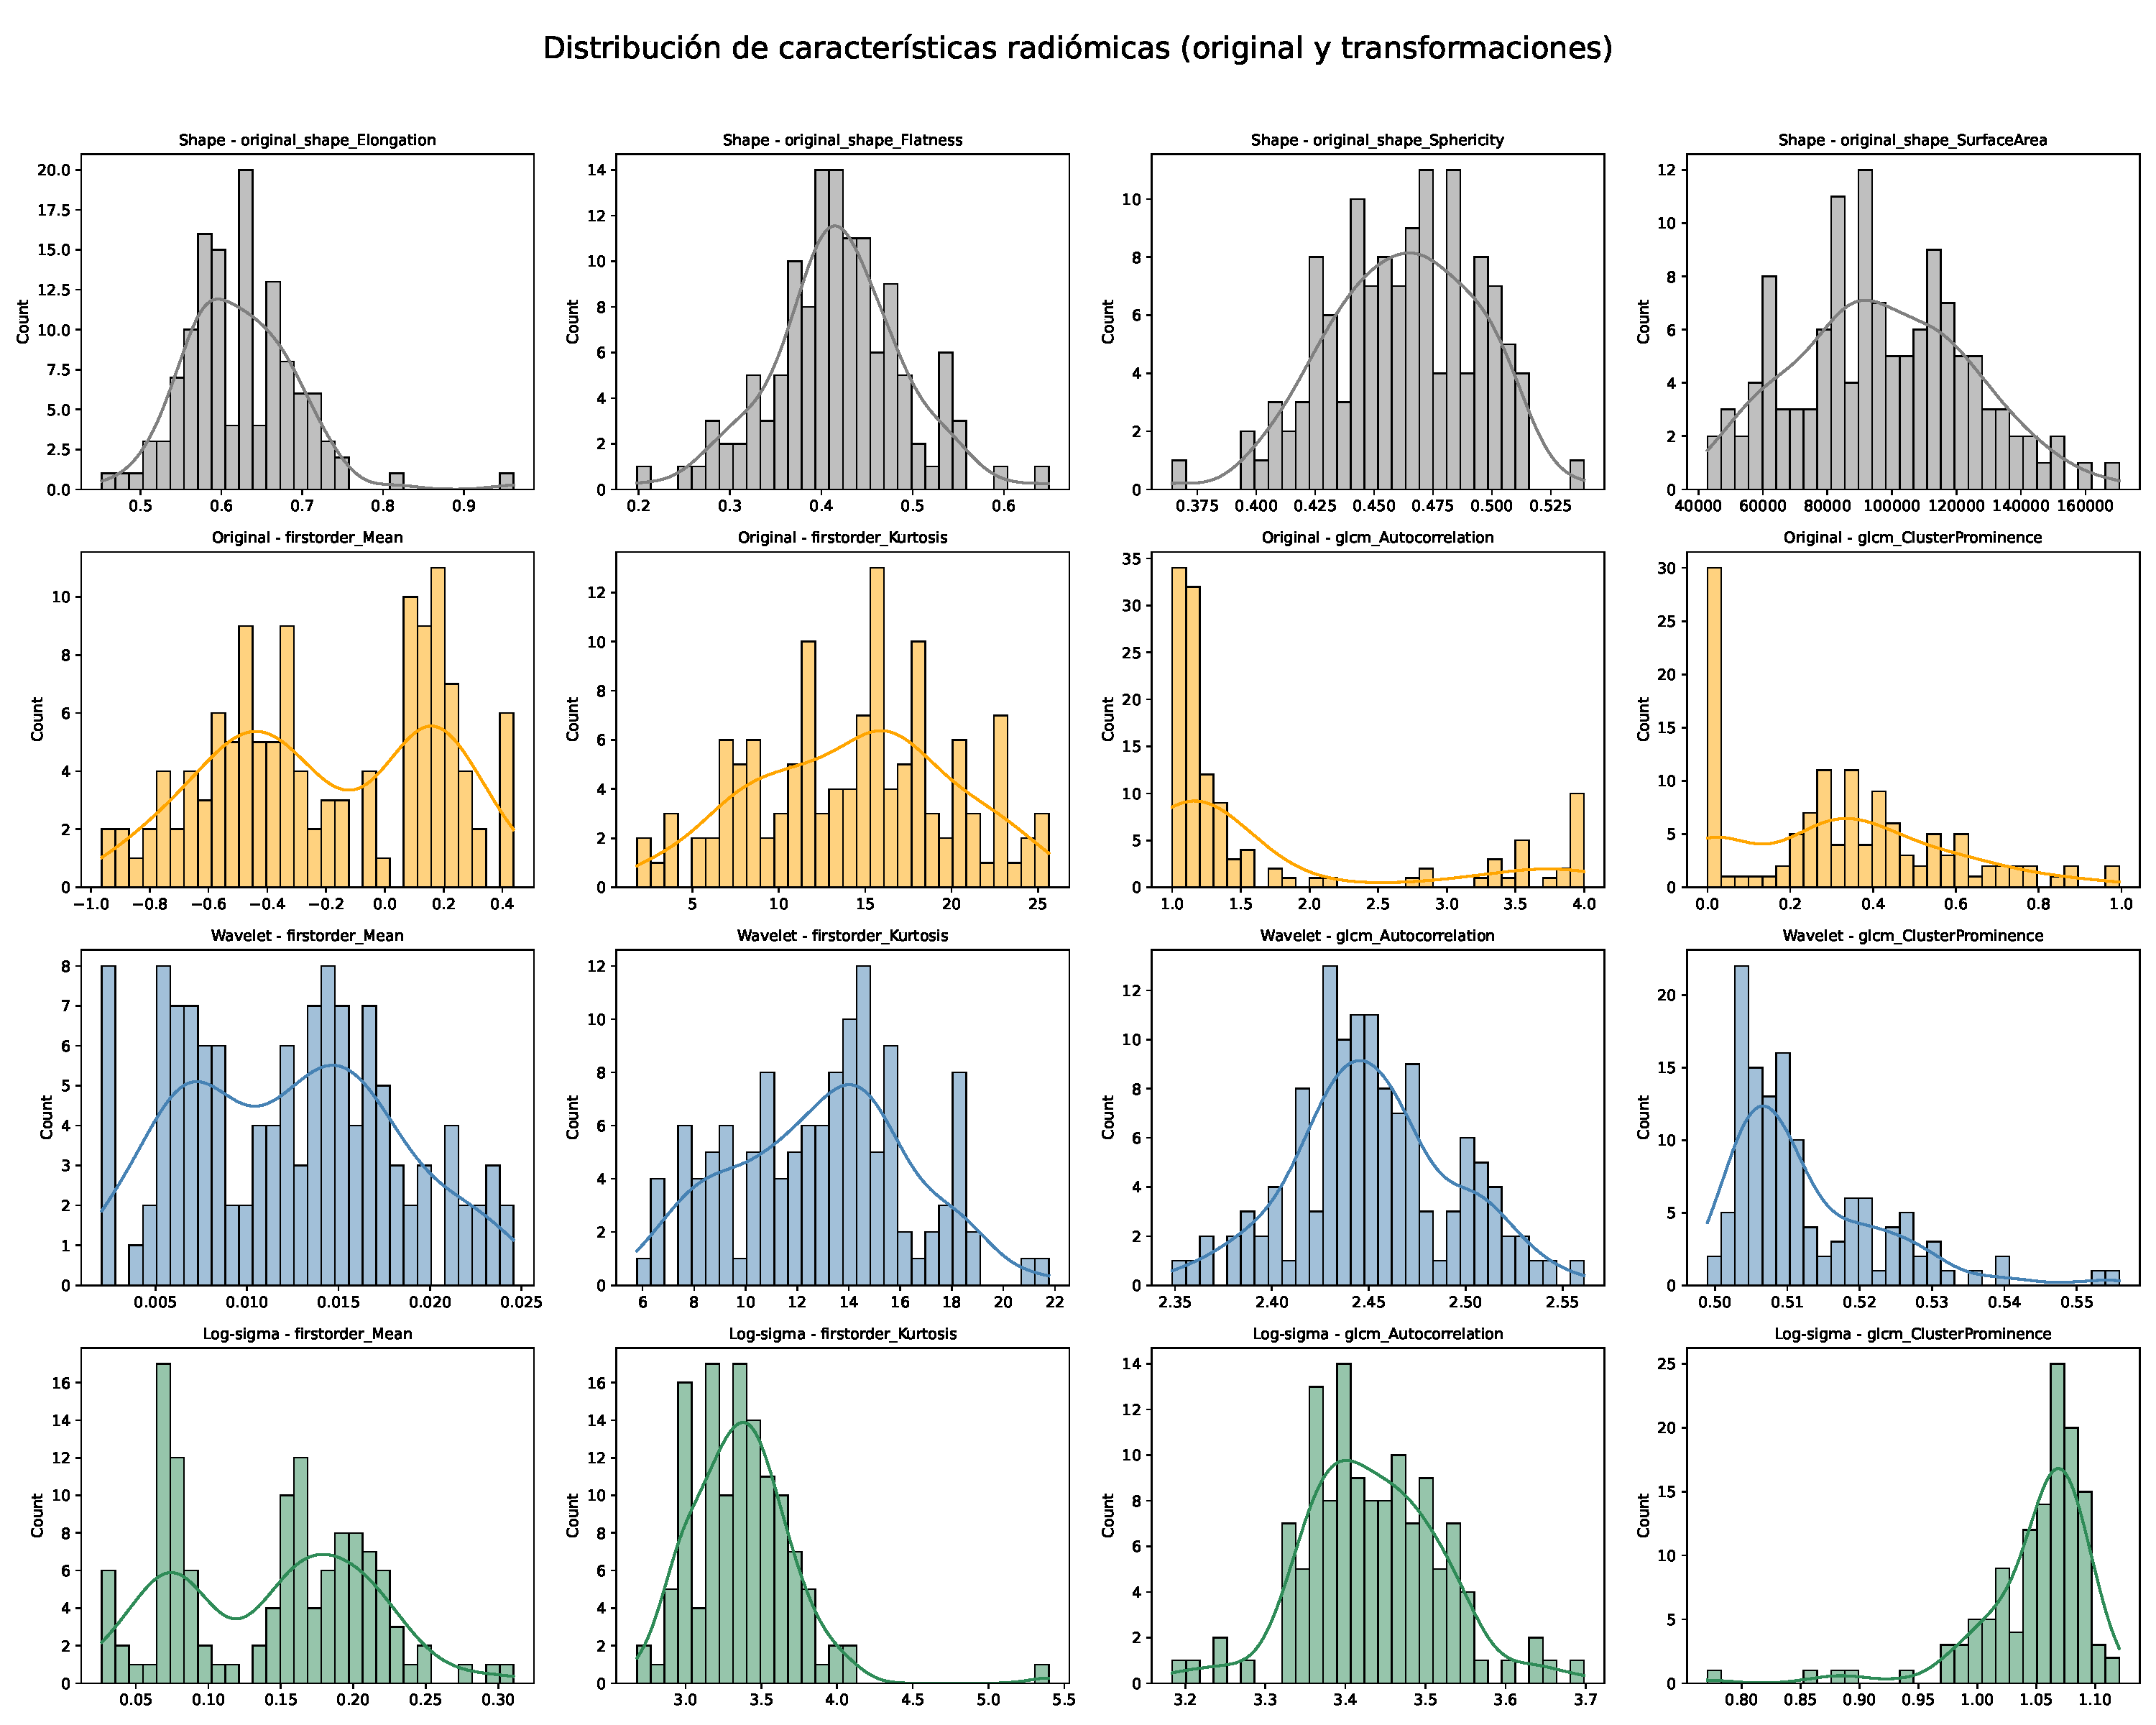
\includegraphics[width=\textwidth]{img/distribucion_features_radiomics.pdf}
\caption{Visualización de distribuciones de algunas características radiómicas. Se muestran tanto atributos de forma, como atributos sin transformar y los mismos atributos sobre las imágenes con filtros wavelet y logarítmicos.}\label{fig:dist_radiomics}
\end{figure}

Otro aspecto interesante a considerar es la correlación entre variables, ya que es posible que muchas características radiómicas estén altamente correlacionadas o incluso sean linealmente dependientes unas de otras. Puede ser el caso de ciertos percentiles de primer orden que se extraen, o ciertos atributos de las matrices de segundo orden. En la Figura \ref{fig:corr_radiomics} visualizamos la matriz de correlación de las características originales. Las extendidas no se muestran debido a su gran tamaño. Podemos observar que, efectivamente, hay muchas variables altamente correladas, tanto positiva como negativamente. Muchas de ellas, de hecho, alcanzan la correlación 1 o -1. No merece la pena tener tantas variables redundantes, así que se ha optado por eliminar, de todos los pares de atributos con correlación 1 o -1, uno de los pares, hasta que la matriz de correlación deje de tomar dichos valores. Se eliminan un total de 18 atributos redundantes entre las características originales, y un total de 585 al usar las características extendidas, dejando los datasets resultantes en unas dimensiones de $125 \times 89$, y $125 \times 1382$, respectivamente. En este último, la reducción es muy significativa, aunque aún sigue teniendo dimensionalidad muy alta. En la Figura \ref{fig:corr_after_remove} se muestra cómo queda la matriz de correlación tras eliminar todas las características redundantes. En ella podemos ver que las celdas con valores extremos disminuyen. Aun así quedan ciertos atributos altamente correlados sin llegar a ser dependientes. Por el momento, se ha optado por preservarlos.

\begin{figure}[!htbp]
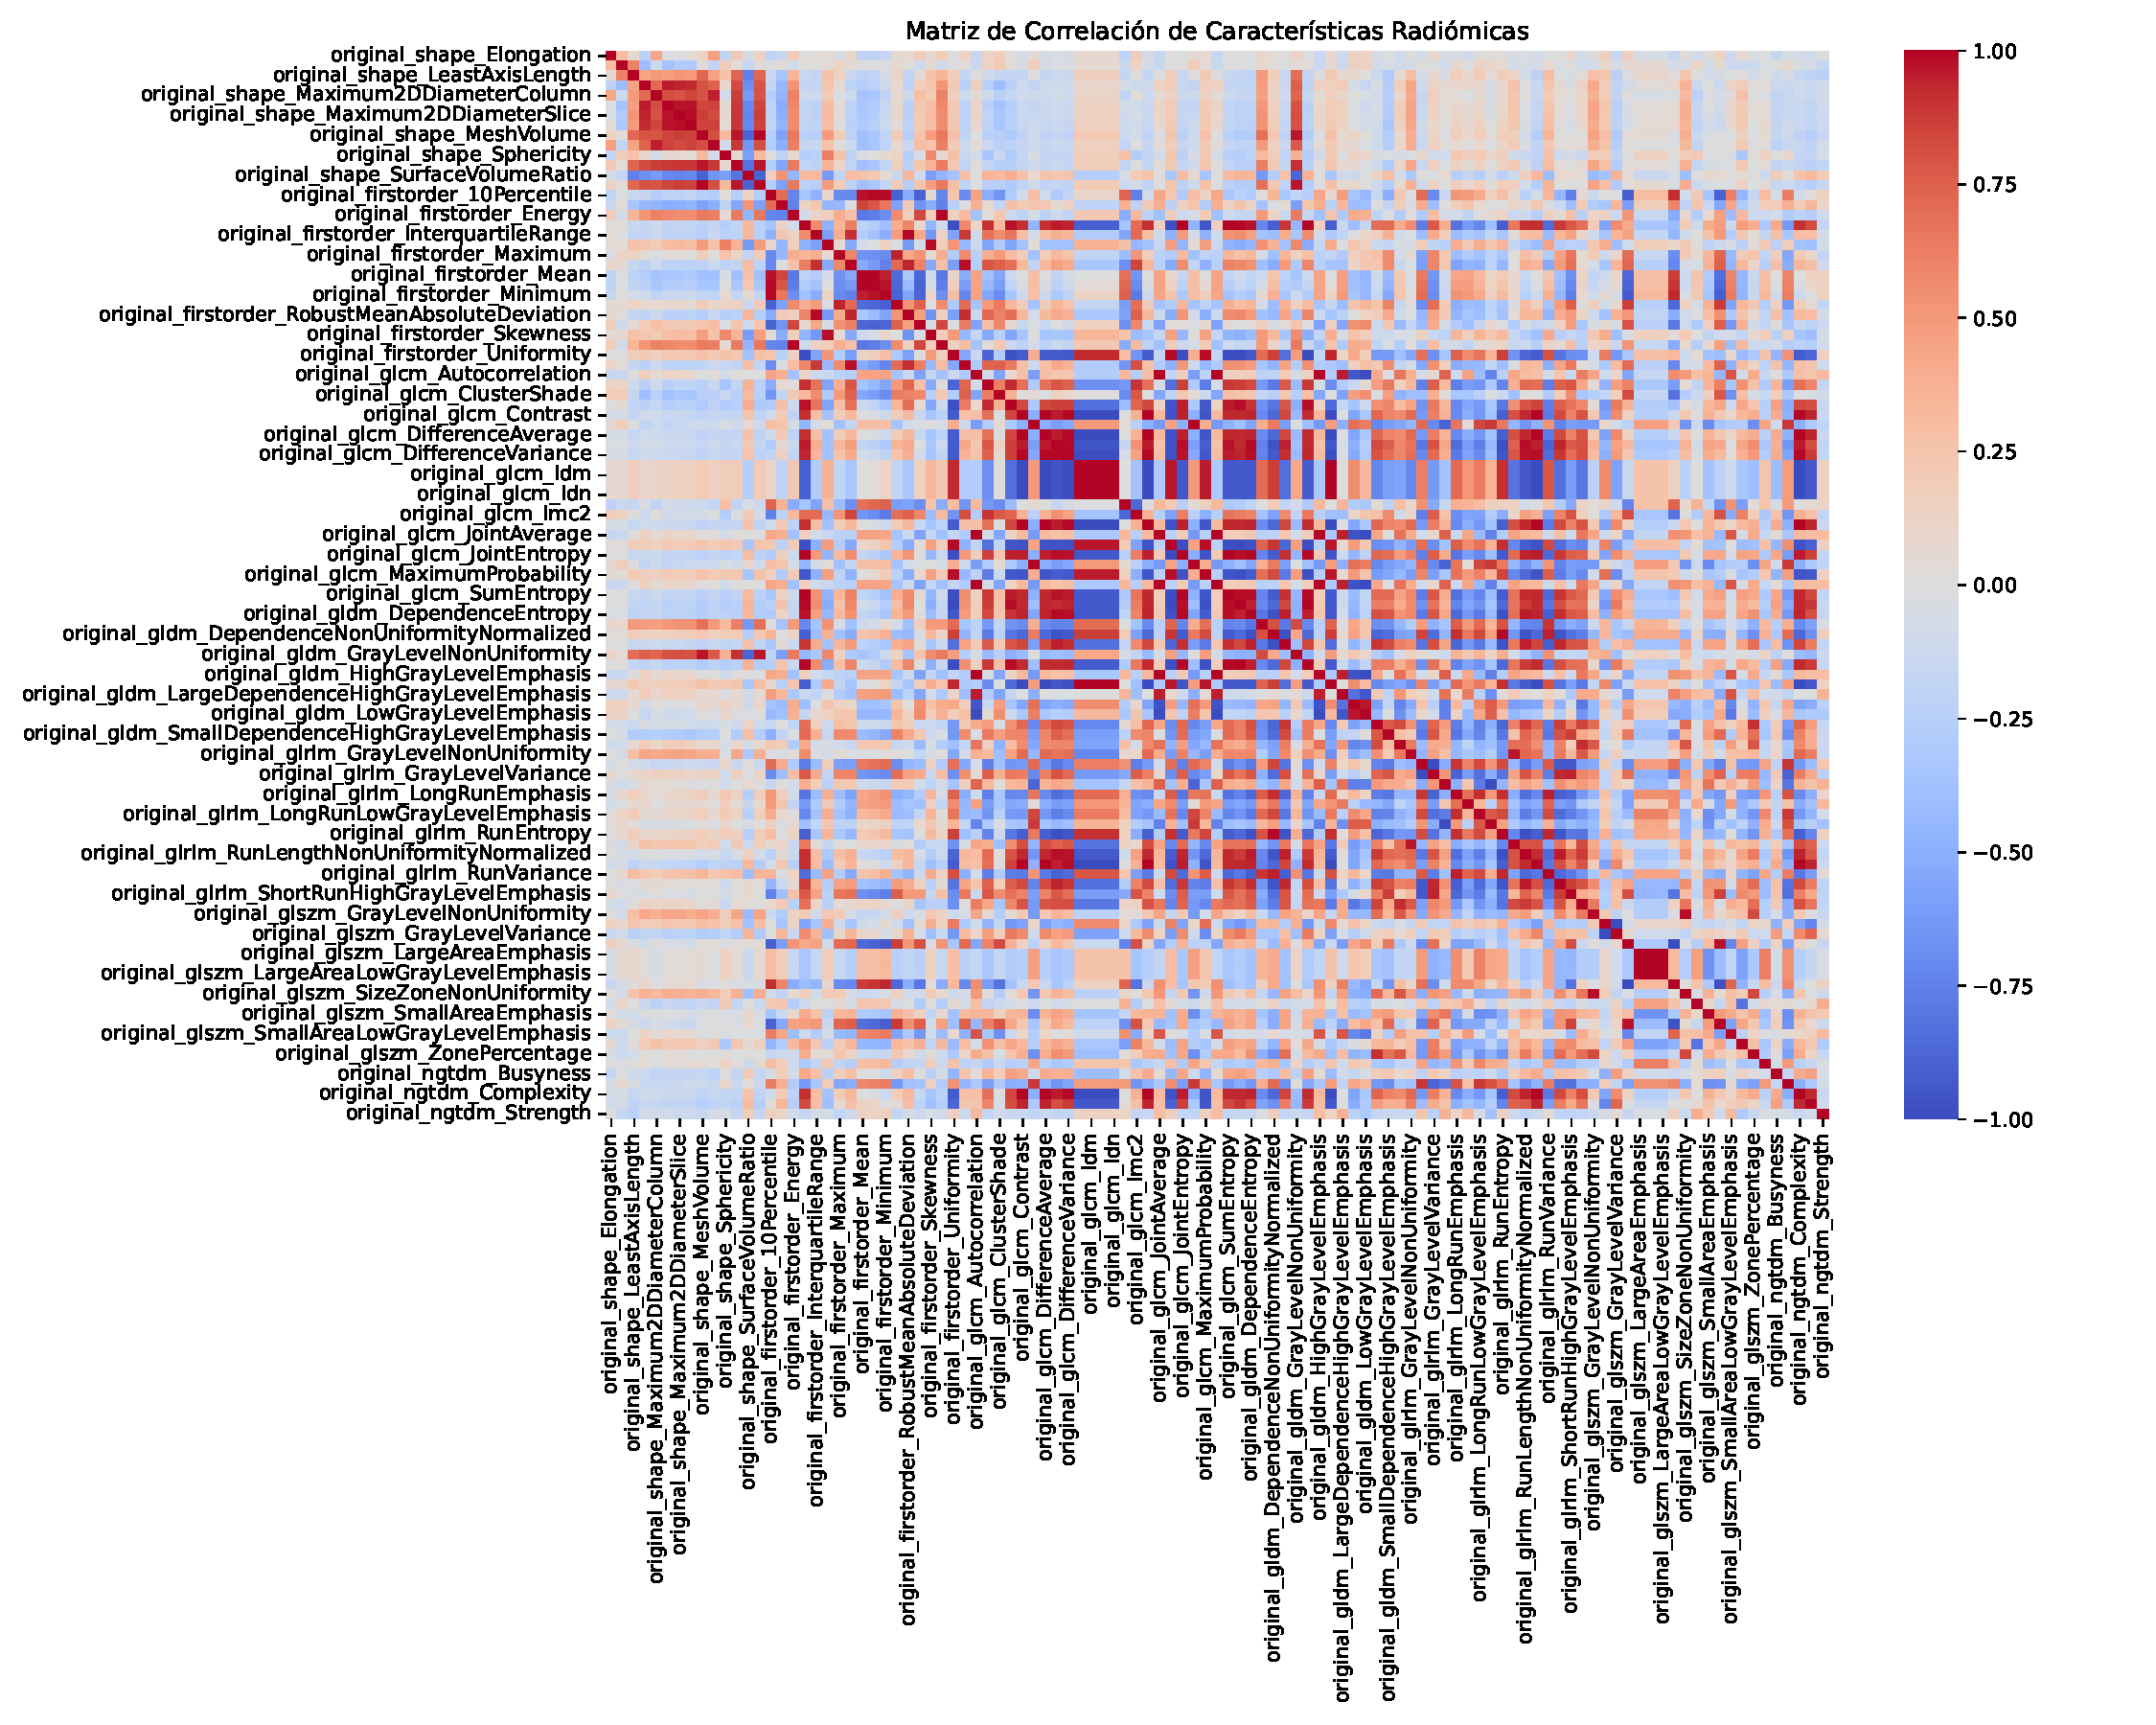
\includegraphics[width=\textwidth]{img/corrplot_radiomics.pdf}
\caption{Matriz de correlación sobre las características radiómicas originales.}\label{fig:corr_radiomics}
\end{figure}

\begin{figure}[!htbp]
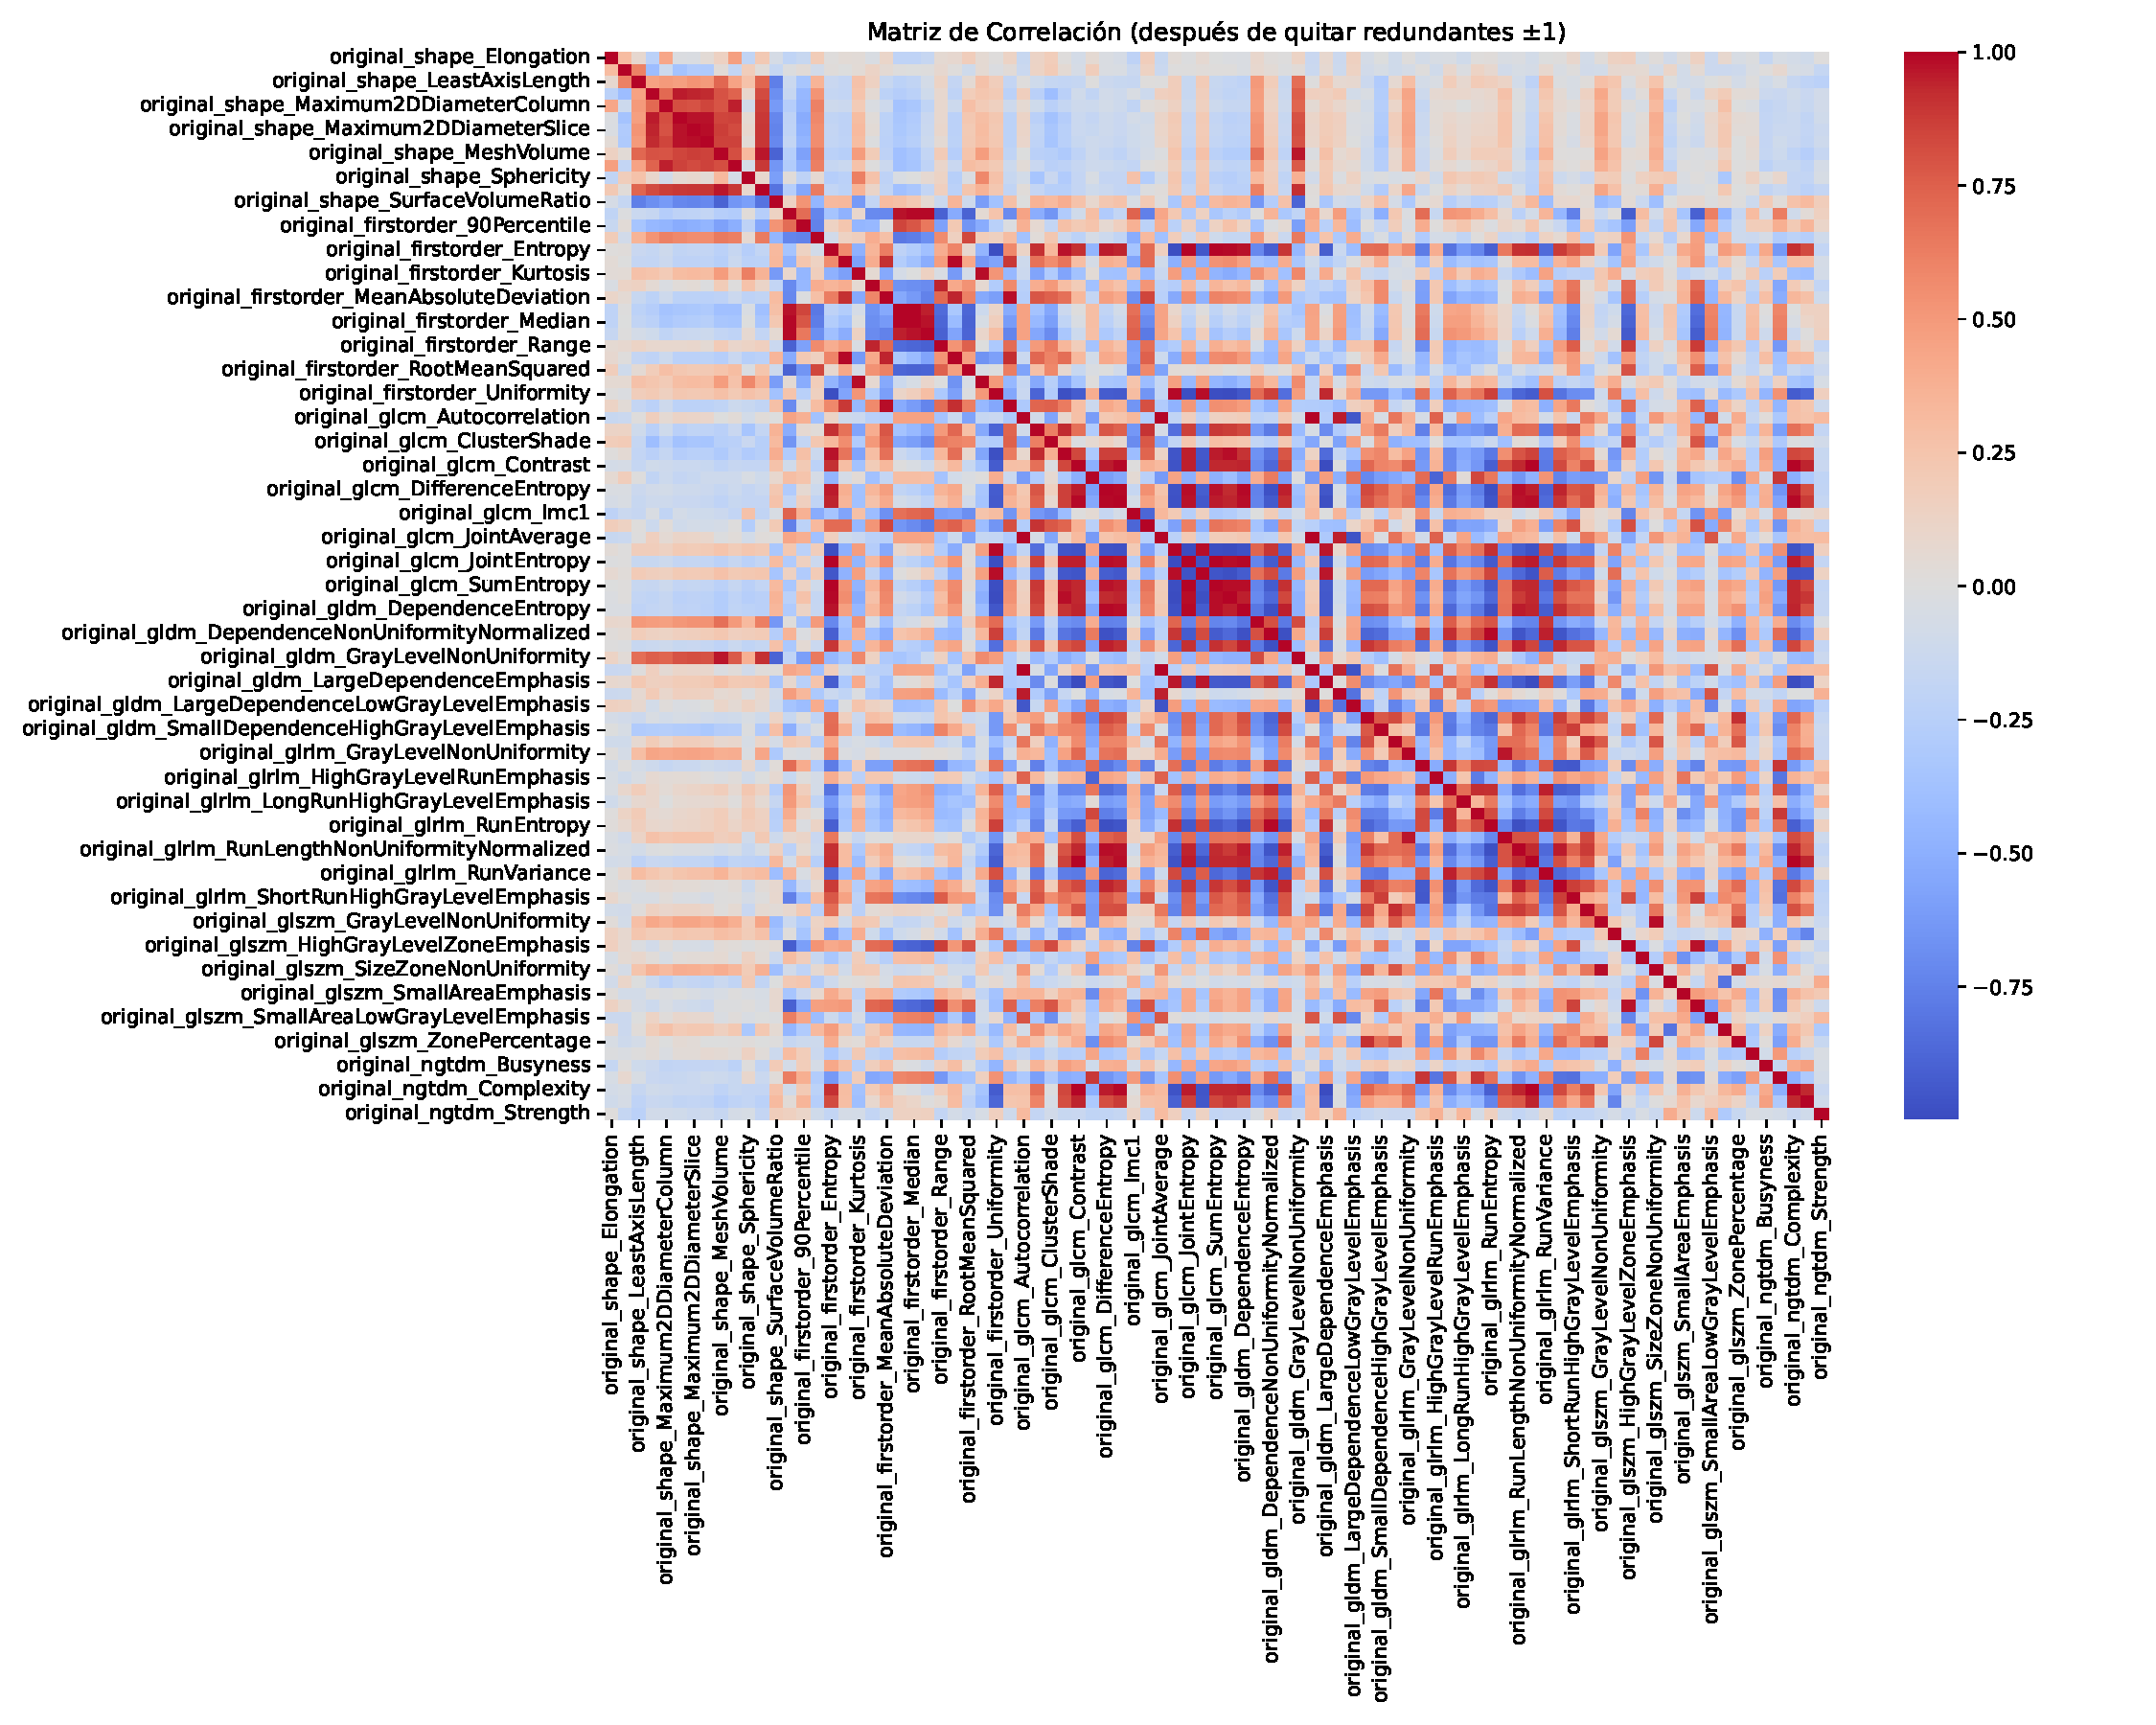
\includegraphics[width=\textwidth]{img/corrplot_radiomics_cleaned.pdf}
\caption{Matriz de correlación sobre las características radiómicas originales tras eliminar variables redundantes.}\label{fig:corr_after_remove}
\end{figure}

Otro aspecto interesante a tener en cuenta es el análisis de una posible correlación con las etiquetas, para tratar de identificar qué atributos pueden tener mayor influencia, individualmente, en la predicción de existencia de complicación. En las Figuras \ref{fig:corr_labels_original} y \ref{fig:corr_labels_extended} se muestran las características más correladas, en valor absoluto, con la etiqueta \emph{Complicación} de las características radiómicas, las originales y las extendidas, respectivamente. Tanto en las originales como en las extendidas, podemos ver que no destaca ninguna variable altamente correlada. En el caso de las extendidas, vemos que las características más correladas se corresponden casi todas con transformaciones \emph{wavelet} en diferentes direcciones, aunque apenas se llega a superar el 0.3 en el mejor caso. Por tanto, no parece que haya dependencias lineales con la clase que buscamos predecir y alguna característica individual.

% \begin{figure}[!htbp]
% \includegraphics[width=\textwidth]{top_features_corr_label_complicacion.pdf}
% \caption{Top 20 de características originales más correladas en valor absoluto con la existencia de complicación.}\label{fig:corr_labels_original}
% \end{figure}

% \begin{figure}[!htbp]
% \includegraphics[width=\textwidth]{ext_top_features_corr_label_tipo_complicacion.pdf}
% \caption{Top 20 de características extendidas más correladas en valor absoluto con la existencia de complicación.}\label{fig:corr_labels_extended}
% \end{figure}

\begin{figure}[!htbp]
    \centering
    \begin{subfigure}[t]{0.48\textwidth}
        \includegraphics[width=\textwidth]{img/top_features_corr_label_complicacion.pdf}
        \caption{Top 20 de características originales más correladas en valor absoluto con la existencia de complicación.}
        \label{fig:corr_labels_original}
    \end{subfigure}
    \hfill
    \begin{subfigure}[t]{0.48\textwidth}
        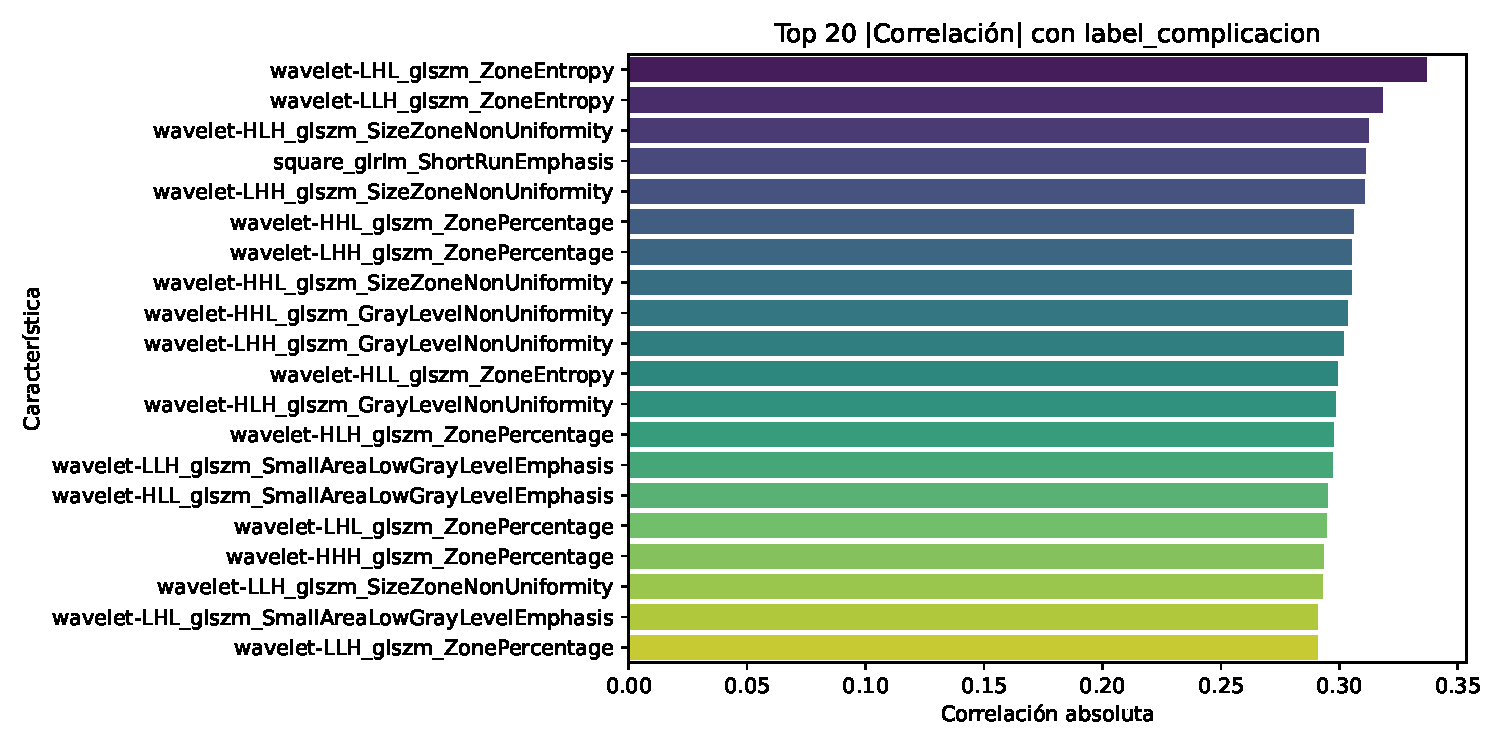
\includegraphics[width=\textwidth]{img/ext_top_features_corr_label_complicacion.pdf}
        \caption{Top 20 de características extendidas más correladas en valor absoluto con la existencia de complicación.}
        \label{fig:corr_labels_extended}
    \end{subfigure}
    \caption{Comparación de las 20 características más correladas con la existencia de complicación en el conjunto original (a) y extendido (b).}
    \label{fig:combined_corr_labels}
\end{figure}



Por último, dada la alta dimensionalidad presente en los datasets aún tras la eliminación de las variables redundantes, se ha optado por aplicar técnicas de selección de instancias y de reducción de dimensionalidad no supervisadas para la obtención de datasets de características más reducidos. Por un lado, se ha optado por aplicar la técnica de selección de características \emph{Variance Threshold}, que busca eliminar atributos con varianza inferior a un umbral pasado como parámetro. En nuestro caso, hemos tomado el umbral 0.01. Por otro lado, se ha utilizado \emph{PCA} como técnica de reducción de dimensionalidad, para obtener un mapeo en un espacio de menor dimensionalidad en el que se preserve la mayor parte de la varianza del dataset (se explican sus detalles en la Sección \ref{sec:pca}). En este caso, se ha optado por quedarse con varias posibilidades: el conjunto de componentes principales con las que se preserva el 99, 95 y 90 \% de la varianza, respectivamente. De cada posibilidad surge un dataset que se ha utilizado para entrenar los modelos de la siguiente sección. En la Tabla \ref{tbl:red_dim} se muestran las dimensionalidades alcanzadas tras aplicar estas técnicas (se muestran para el caso actual, para el resto de tamaños y ventanas el procedimiento es análogo y se consiguen resultados similares). Podemos ver que, especialmente, con las características extendidas, se reduce la dimensionalidad rápidamente, incluso con un PCA preservando el 99 \% de la varianza, lo que nos indica que puede que sea posible resumir la información de las características extendidas en 68 dimensiones sin perder demasiada información.

\begin{table}[!htbp]
\centering
\begin{tabular}{lcc}
\hline
 & \textbf{Original} & \textbf{Extendido} \\
\hline
Dimensión inicial       & 107 & 1967 \\
Sin redundantes         & 89  & 1382 \\
Variance Threshold      & 79  & 588  \\
PCA 99\%                 & 23  & 68   \\
PCA 95\%                 & 14  & 33   \\
PCA 90\%                 & 10  & 20   \\
\hline
\end{tabular}
\caption{Reducción de dimensionalidad para los conjuntos con características originales y extendidas obtenidas a partir del dataset de tamaño $128\times 256 \times 256$ sin aplicar ventanas Hounsfield.}
\label{tbl:red_dim}
\end{table}


\section{Entrenamiento de modelos de aprendizaje automático}

Finalmente, sobre los distintos datasets obtenidos con los procedimientos anteriores, se han probado distintos algoritmos de aprendizaje automático. Se han seleccionado algoritmos de diferente naturaleza para experimentar:

\begin{itemize}
    \item \textbf{Regresión logística.} Un algoritmo rápido y eficiente que, aunque en principio no se espera que logre buenos resultados, puede ayudar a hacernos una idea sobre la separabilidad lineal de los datos.
    \item \textbf{Árboles de decisión.} Otro algoritmo sencillo que posiblemente tampoco alcance buenos resultados, pero en caso afirmativo podría proporcionar interpretabilidad a los resultados.
    \item \textbf{SVM.} Las máquinas de vectores soporte son algoritmos robustos que además pueden adaptarse a distintas estructuras del conjunto de datos utilizando el kernel adecuado.
    \item \textbf{$k$-NN.} El algoritmo de los $k$ vecinos más cercanos puede ser efectivo si la representación espacial de los datos radiómicos es buena. Además, no tiene parámetros que aprender. Por otra parte, puede verse perjudicado especialmente por los conjuntos de datos de mayor dimensionalidad.
    \item \textbf{Ensembles.} Los ensembles suelen ser los algoritmos de aprendizaje automático clásico más efectivos en cuanto a capacidad de aprendizaje. Se ha optado por probar varios tipos de ensembles, tanto basados en bagging, como es el caso de los \emph{random forest}, como basados en boosting, para lo que se han seleccionado los algoritmos \emph{LightGBM}, \emph{XGBoost} y \emph{Gradient Boosting}.
\end{itemize}

El reducido número de instancias en nuestro conjunto de datos ha permitido la ejecución de múltiples versiones de los algoritmos variando parámetros. Por ejemplo, para el $k$-NN se han probado distintos números de $k$, en SVM distintos tipos de kernels y en los ensembles distinta cantidad de clasificadores débiles, entre otros. Los detalles de la experimentación se describirán en la Sección \ref{sec:experimentos}.

También es importante destacar que se ha experimentado con distintos tipos de normalización de los datos, previa a la ejecución de los algoritmos. Se han usado tanto la normalización estándar o Z-score, consistente en restar la media y dividir por la desviación típica, como la normalización \emph{MinMax}, que ajusta los rangos de todos los atributos al intervalo $[0, 1]$. La normalización es especialmente relevante en algoritmos basados en distancias, como el $k$-NN o las SVM.

Por último, se han probado dos modalidades de entrenamiento diferentes: entrenar solo con los datos radiómicos, y entrenar conjuntamente con los datos radiómicos y clínicos. En este último caso, los datos clínicos se incorporan al conjunto de radiómicos antes de realizar las normalizaciones de los datos, para que atributos como la edad del paciente sean normalizados posteriormente, y todas aquellas características clínicas nominales que numerizan con un \emph{one-hot encoding}.

\section{Aprendizaje de métricas de distancia}

Para concluir este capítulo, nos centramos en un caso especial observado durante los resultados de las experimentaciones anteriores. Estos resultados se pueden consultar en la Sección \ref{sec:resultados}. En dicha sección, se puede observar que el $k$-NN, junto con los ensembles, es el algoritmo que más destaca, obteniendo algunos de los mejores resultados. Dichos resultados se obtienen usando la distancia euclídea, que es una distancia estándar que considera a todos los atributos con la misma importancia. Por ello, nos planteamos el intentar mejorar estos resultados aprendiendo una distancia a partir de los datos, y usar dicha distancia posteriormente en el $k$-NN.

Para ello, recurrimos a las técnicas de aprendizaje de métricas de distancia descritas en la Sección \ref{sec:dist}. Concretamente, aplicaremos los siguientes algoritmos LMNN y NCA. Ambos algoritmos están diseñados específicamente para mejorar el rendimiento del $k$-NN, y las transformaciones que aprenden pueden utilizarse para definir una reducción de dimensionalidad con información supervisada, a diferencia de las técnicas aplicadas anteriormente. 

Ambos algoritmos se han aplicado a los conjunto de características originales eligiendo distintos valores como dimensión de salida: 10, 20, 30 y la dimensión completa. Con ello se ha buscado obtener nuevas representaciones del conjunto de datos en las que el algoritmo $k$-NN pudiera alcanzar un mayor rendimiento, y así superar el mejor resultado global alcanzado en este problema.

Al igual que en el entrenamiento sin aprendizaje de métricas de distancias, también se prueba en este caso la incorporación de los datos clínicos. En este caso, los datos se incorporan antes del aprendizaje de las distancias, para que se vean afectados también por la transformación que aprendan los algoritmos.

\endinput
%--------------------------------------------------------------------
% FIN DEL CAPÍTULO. 
%--------------------------------------------------------------------
